\clearpage
\section{The Wishart process}\label{sec:wishart-process}
%%%%%

\info[inline]{Paragraph: Introduce Wishart process and its history and application.}
In this section, we introduce the \gls{wp} to the task of estimating \gls{tvfc}.
Described by \textcite{Bru1991} as matrix generalizations of square Bessel processes, the \gls{wp} is a stochastic matrix process consisting of (for our intents and purposes) covariance matrices.
\textcite{Wilson2010} described a more modern and generalized version of this stochastic process.
%
We discuss its basic construction as well as any required adaptation and fine-tuning to the field of neuroimaging.
We note that many additional improvements and tweaks are still possible, and promising future work directions are discussed in \cref{subsec:model-extensions}.
Model parameters are inferred through \gls{vi}, an approximate inference routine.
The promise of \glspl{wp} is presented by \textcite{Wilson2010, Heaukulani2019} as well, where it is shown that it outperforms \gls{mgarch} models on a range of data sets.

As we enter the domain of Bayesian machine learning~\parencite{Ghahramani2015}, familiarity with concepts from excellent textbooks such as \textcite{MacKay2002, Bishop2006, Hastie2009, Murphy2012, Murphy2023} will prove helpful.

%%
\subsection{The Wishart distribution}\label{subsec:wishart-distribution}
%%

\info[inline]{Paragraph: Introduce Wishart distribution.}
The Wishart \emph{distribution} defines a probability density function over $D \times D$ symmetric positive definite matrices $\mathbf{\Sigma}$:
\begin{equation}
  f(\mathbf{\Sigma}|\mathbf{V},\nu) = \frac{1}{Z} |\mathbf{\Sigma}|^{(\nu - D - 1)/2} \exp{(-\frac12tr(\mathbf{V}^{-1}\mathbf{\Sigma}))},
\end{equation}
where $\mathbf{V}$ is a $D \times D$ positive definite scale matrix, and $\nu \geq D$ is the number of degrees of freedom.
The normalization constant $Z$ is given by $2^{\nu D/2}|\mathbf{V}|^{\nu/2}\Gamma_D(\nu/2)$, where $\Gamma_D(\cdot)$ is the multivariate gamma function:
\begin{equation}
  \Gamma_D(\nu/2) = \pi^{D(D-1)/4} \prod_{j=1}^D \Gamma(\nu/2 + (1-j)/2).
\end{equation}
This distribution has mean $\nu \mathbf{V}$ and mode $(D - \nu - 1)\mathbf{V}$ for $\nu \geq D + 1$.

\info[inline]{Paragraph: Discuss Wishart distributed matrix construction.}
Crucially, we can construct a Wishart-distributed random (matrix-valued) variable from a collection of i.i.d.~zero-mean Gaussian random variables.
Namely, the sum of outer products of multivariate Gaussian random variables is Wishart distributed:
\begin{equation}
  \mathbf{\Sigma} = \sum_{i=1}^\nu \textbf{u}_i \textbf{u}_i^T \sim \mathcal{W}_D(\mathbf{V}, \nu),
  \label{eq:wishart-from-iid-gaussians}
\end{equation}
where $\textbf{u}_i$ are i.i.d. $\mathcal{N}(\textbf{0}, \mathbf{V})$ distributed, $D$-dimensional random variables.
$\mathcal{W}_D(\mathbf{V}, \nu)$ denotes a Wishart distribution with $D \times D$ scale matrix $\mathbf{V}$, and $\nu$ degrees of freedom.
We use this property to construct the \gls{wp}.
A matrix constructed in this manner will always be a valid covariance matrix: symmetric and positive semi-definite.

%%
\subsection{Wishart process model definition}
%%

\info[inline]{Paragraph: Define Wishart process model construction.}
For the \gls{wp} definition, we follow the notations from~\textcite{Heaukulani2019}.
Let $Y$ := ($\mathbf{y}_n$, $1 \leq n \leq N$) denote a sequence of measurements in $\mathbb{R}^D$.
That is, $\mathbf{y}_n = [y_{n,1}, \dots, y_{n,D}]$.
In \gls{fmri} analyses, $N$ refers to the number of time steps or scan \emph{volumes}, and $D$ refers to the number of node time series (e.g.~number of brain regions for which a characteristic \gls{bold} signal time series is determined).

We denote \textbf{input locations} as $X$ := ($x_n$, $1 \leq n \leq N$) in $\mathbb{R}$.
For \gls{fmri} analyses, the (univariate, 1-dimensional)~$x_n$ here is the time at which measurement $\mathbf{y}_n$ is taken (observed).\footnote{Our model construction does not \emph{require} the input locations to be univariate. One could, for example, add other (side) information of interest such as the decaying magnet strength during a scan, head motion~\parencite[often considered one of the most significant confounding factors, see e.g.][]{Laumann2017}, a design matrix for \gls{tb-fmri}, arousal (e.g.~as measured by pupil diameter or eyelid closure), and/or physiological signals such as heart rate. Whether this is beneficial will require further validation studies.}
In our model definition the spacing between values of $x_n$ may be irregular and does not need to be constant.
Even though we expect \gls{fmri} data to be organized in a grid-like fashion of regular time intervals of a single \gls{tr}, this model flexibility could still be useful.
For example, it allows for naturally leaving out a measurement due to an artifact.
From the Bayesian perspective, we just so happen to make \emph{observations} at fixed intervals (giving the impression of a state-space structure), but this may not reflect the underlying process.
For computational ease-of-use, we consider $X$ (the scan frame times) in the fixed interval of [0, 1] during training and prediction.
Estimates are then scaled back to the scan time frame.

We let the conditional likelihood of observations be multivariate Gaussian:
\begin{equation}
  \mathbf{y}_n \mid \boldsymbol{\mu}_n, \mathbf{\Sigma}_n \sim \mathcal{N}(\boldsymbol{\mu}_n, \mathbf{\Sigma}_n),
\end{equation}
where $\mathbf{\Sigma}_n$ is a $D \times D$ covariance matrix.
This is a researcher choice; other likelihood functions such as the multivariate $t$-distribution could be implemented instead.
In dealing with \gls{fmri} data, we may assume all entries of the mean vector~$\boldsymbol{\mu}_n$ to be zero, so this likelihood simplifies to
\begin{equation}
  \mathbf{y}_n \mid \mathbf{\Sigma}_n \sim \mathcal{N}(\textbf{0}, \mathbf{\Sigma}_n).
\end{equation}
In our context, we are not interested in the actual values of $\mathbf{y}_n$.
Instead, we are interested in the (random) process $\mathbf{\Sigma}_1, \mathbf{\Sigma}_2, \dots, \mathbf{\Sigma}_N$.
This process constitutes the \gls{tvfc} as described in \cref{sec:tvfc}.
Again, this covariance process (or \emph{structure}) is never directly observed.

As mentioned before, a Wishart distributed random (matrix-valued) variable can be constructed from i.i.d.\ collections of Gaussian random variables.
Analogously, we can construct \glspl{wp} from i.i.d.~collections of Gaussian \emph{processes}~\parencite{Rasmussen2006}.\footnote{\textcite{Gourieroux2009} construct \glspl{wp} is a similar fashion, but instead of \glspl{gp} they use (stochastic) vector autoregressive processes as underlying latent processes.}
Let
\begin{equation}
  f_{d,k} \sim GP(\textbf{0}, \mathcal{K}(\cdot, \cdot ; \theta)),
\end{equation}
for $1 \leq d \leq D$ and $1 \leq k \leq \nu$, where $\mathcal{K}(\cdot, \cdot ; \theta)$ refers to a \emph{kernel} function (a.k.a.~covariance function) with respective kernel parameters $\theta$.
It is our job as modelers to choose a suitable kernel function.

Evaluating a \gls{gp} at a given point in time returns a Gaussian distributed random variable.
Let $F_{n,d,k} := f_{d,k}(X_n)$ denote the evaluation of the \gls{gp} at point $X_n$.
Under the posterior this is \emph{not} a zero-mean Gaussian variable anymore.
Moreover, unlike with a \gls{gp}, the posterior of the \gls{wp} is \emph{not} a \gls{wp}.

We write $\mathbf{F}_n$ for the aggregate (random) $D \times \nu$ matrix $(F_{n,d,k})_{1\leq d\leq D,1\leq k\leq \nu}$, which has entries $F_{n,d,k}$, indexed by $d$ and $k$.
Analogues to \cref{eq:wishart-from-iid-gaussians}, we can then construct
\begin{equation}
\label{eq:sigma-definition}
  \mathbf{\Sigma}_n = \mathbf{A} \mathbf{F}_n \mathbf{F}_n^T \mathbf{A}^T
\end{equation}
as a Wishart-distributed random matrix at time $n$.

This construction allows us to query at any point in time, as the underlying \glspl{gp} can be queried at any value of $x_n$.
We make sure $\mathbf{A} \in \mathbb{R}^{D \times D}$ is restricted so that \emph{scale matrix} $\mathbf{A}\mathbf{A}^T$ is positive definite.
Recall that $\mathbf{A}\mathbf{A}^T$ corresponds to the scale matrix $\mathbf{V}$ as discussed in \cref{subsec:wishart-distribution}.
That is, $\mathbf{A}$ is the Cholesky factor of $\mathbf{V}$.
The scale matrix covariance terms can be considered mean covariances across the time series.
We train matrix $\mathbf{A}$ as part of the inference routine.
Intuitively, for a static covariance estimate, our \gls{wp} could simply learn these $\mathbf{A}$ covariance terms and `switch off' the \glspl{gp}.

Writing it out, our zero-mean, multivariate Gaussian likelihood is given by
\begin{equation}
  p(\mathbf{y}_n|\mathbf{\Sigma}_n) = \frac{1}{(2\pi)^{\frac{D}{2}} |\mathbf{\Sigma}_n|^{\frac{1}{2}}} e^{-\frac{1}{2} \mathbf{y}_n \mathbf{\Sigma}_n^{-1} \mathbf{y}_n}.
\end{equation}
Plugging in our construction of $\mathbf{\Sigma}_n$ from \cref{eq:sigma-definition}, we obtain
\begin{equation}
  p(\mathbf{y}_n|\mathbf{A},\mathbf{F}_n) = \frac{1}{(2\pi)^{\frac{D}{2}} |\mathbf{A} \mathbf{F}_n \mathbf{F}_n^T \mathbf{A}^T|^{\frac{1}{2}}} e^{-\frac{1}{2} \mathbf{y}_n (\mathbf{A} \mathbf{F}_n \mathbf{F}_n^T \mathbf{A}^T)^{-1} \mathbf{y}_n}.
\end{equation}
The log of this likelihood is given by
\begin{equation}
  \log p(\mathbf{y}_n|\mathbf{A},\mathbf{F}_n) = - \frac{D}{2} \log 2\pi - \frac{1}{2} \log |\mathbf{A} \mathbf{F}_n \mathbf{F}_n^T \mathbf{A}^T| - \frac{1}{2} \mathbf{y}_n^T (\mathbf{A} \mathbf{F}_n \mathbf{F}_n^T \mathbf{A}^T)^{-1} \mathbf{y}_n.
\end{equation}

In Bayesian model definition, apart from a likelihood, we have to choose a prior.
We choose a fully factorized prior over $F$.
This is typically considered a fair assumption, as independence in the prior does not lead to independence in the posterior.
That is,
\begin{equation}
  p(F) = \prod_{n=1}^N p(\mathbf{F}_n) = \prod_{n=1}^N \left[ \prod_{d=1}^D \prod_{k=1}^\nu f_{d,k}(X_n) \right].
\end{equation}

We know that $Y_n$ only depends on $\mathbf{F}_n$, so $p(Y|F) = \prod_{n=1}^N p(\mathbf{y}_n|\mathbf{A},\mathbf{F}_n)$.
Since all entries of $\mathbf{F}_n$ are~i.i.d., we can write
\begin{equation}
  p(Y,F) = p(Y|F)p(F) = \prod_{n=1}^N \left[ p(\mathbf{y}_n|\mathbf{A},\mathbf{F}_n) \prod_{d=1}^D \prod_{k=1}^\nu f_{d,k}(X_n) \right].
\end{equation}

Recall that we want correlation in $Y$.
With independence in $\mathbf{F}_n$, we do get such correlation in $\mathbf{\Sigma}$.

%%
\subsection{Variational Wishart processes}
%%

\info[inline]{Paragraph: Describe (variational) inference routine.}
We are interested in the posterior
\begin{equation}
  p(F|Y) = \frac{p(Y,F)}{p(Y)},
\end{equation}
where computing $p(Y) = \int p(Y|F)p(F)dF$, the marginal density of observations or \emph{evidence}, is intractable.
We therefore resort to \textbf{approximate inference} routines.

\Gls{vi} is a technique that approximates a probability density through \emph{optimization}~\parencite{Jordan1999, Hoffman2015, Blei2017}.
It is usually faster and more scalable than other inference methods, such as \gls{mcmc} sampling~\parencite[as used in e.g.][]{Fox2011}, especially with larger data sets.
In fact, the recent advances that made this style of inference possible explain the `why now' of introducing this model to the task of \gls{tvfc} estimation.

With \gls{vi}, we posit a family of distributions~$q(F)$ over the latent variables and then find the member of that family which is close to the target distribution (the true posterior)~$p(F|Y)$.
Closeness here is measured by \gls{kl-divergence}.
The key is to define this family~$q(F)$ to be flexible enough to capture a density close to the posterior, but simple enough for efficient optimization.

We collectively denote $F_{d,k} := (F_{n,d,k}, n \leq N)$.
We choose the variational approximation to the posterior distribution of the latent variables to take the following form:
\begin{equation}
  q(F_{d,k}) \sim \mathcal{N}(F_{d,k};\boldsymbol{\mu}_{d,k}, \mathbf{S}_{d,k}),
\end{equation}
for some \textbf{variational parameters} $\boldsymbol{\mu}_{d,k} \in \mathbb{R}^N$ and $\mathbf{S}_{d,k} \in \mathbb{R}^{N \times N}$ a real, symmetric, positive definite matrix.
We train these parameters together with $\mathbf{A}$ and kernel parameters $\theta$.

Recall that \gls{kl-divergence} is defined as
\begin{equation}
  \operatorname{KL}(q(F)~\|~p(F | Y)) = \mathbb{E}_{q(F)}[\log q(F)] - \mathbb{E}_{q(F)}[\log p(F | Y)].
\end{equation}
Expanding the conditional, we can write
\begin{equation}
  \operatorname{KL}(q(F)~\|~p(F | Y)) = \mathbb{E}_{q(F)}[\log q(F)] - \mathbb{E}_{q(F)}[\log p(F, Y)] + \log p(Y)
\end{equation}
In \gls{vi} we optimize the \gls{elbo}, which is equivalent to this \gls{kl} term up to an added constant:
\begin{equation}
  \begin{split}
    ELBO & = \mathbb{E}_{q(F)}[\log p(F, Y)] - \mathbb{E}_{q(F)}[\log q(F)] \\
    & = \mathbb{E}_{q(F)}[\log p(Y|F)] - \operatorname{KL}(q(F)~\|~p(F)).
  \end{split}
\end{equation}

The first term of the \gls{elbo} is a likelihood (model fit) term and the second term encourages densities close to the prior (i.e.~it can be considered a complexity penalty).

We make a \emph{mean-field} (fully factorized) simplification for $q(F)$:
\begin{equation}
  q(F) = \prod_{d=1}^D \prod_{k=1}^\nu q(F_{d,k}).
\end{equation}
Our \gls{elbo} is then given by
\begin{equation}
  ELBO = \sum^N_{n=1} \mathbb{E}_{q(\mathbf{F}_n)} [\log p(Y_n|\mathbf{F}_n)] - \sum^D_{d=1} \sum^\nu_{k=1} \operatorname{KL}(q(F_{d,k})~\|~p(F_{d,k})).
\end{equation}

We iteratively maximize this as our objective function, using gradient descent.
In order to be able to compute (approximate) gradients we use the `reparameterization trick' as discussed in \textcite{Salimans2013, Kingma2014}.
This boils down to taking samples (Monte Carlo estimates) of our objective function and computing gradients based on these.

%%
\subsection{Additive white noise model}
%%

\info[inline]{Paragraph: Discuss why and how we need to add white noise.}
Following \textcite{Heaukulani2019}, we introduce additive white noise to make inference more robust.
We empirically validated that this is a necessary step to ensure robust inference.
A small amount of noise is added to $f_n$, to avoid values blowing up when $f_n$ is close to zero when taking the inverse.
This means we redefine and update the covariance matrix of $\mathbf{y}_n$ from \cref{eq:sigma-definition} slightly as
\begin{equation}
  \mathbf{\Sigma}_n = \mathbf{A} \mathbf{F}_n \mathbf{F}_n^T \mathbf{A}^T + \mathbf{\Lambda},
\end{equation}
where $\mathbf{\Lambda}$ is the additive noise matrix; a diagonal $D \times D$ matrix with positive (diagonal) entries.
Diagonal values are initialized as 0.01 and are trained with the rest of the before-mentioned model parameters (off-diagonal values remain zero).
This modification may be interpreted as introducing white (or \emph{observational}) noise to the model.

%%
\subsection{Sparse variational Wishart processes}\label{subsec:svwp}
%%

The beauty of basing our \gls{wp} construction on underlying \glspl{gp}, is that we can take advantage of the rapid development and improvement of these models~\parencite[echoing sentiments from][]{Foti2019}.

\glspl{gp} are known to not scale well with large data sets~\parencite{Rasmussen2006}.
When $N$ is large,\footnote{The official \texttt{GPflow} documentation defines `large' as $N > 1000$.} a popular approach to make such models more computationally viable is to use \emph{sparse} variational \glspl{gp}~\parencite{Titsias2009, Hensman2013, Matthews2016}.
These introduce the concept of \emph{inducing points}~\parencite{Bauer2016}.
Such points can be considered learned, auxiliary data points (a.k.a.~pseudo-inputs).
The number of inducing points ($M$) is typically much smaller than $N$.
After training, the model only uses said points to infer and make predictions, rendering a trained model \emph{independent} from the training data.
This approach thus assumes that there is redundant information in the data set.

In \gls{fmri} scans, the size of $N$ tends not to be problematic, as the time needed to take a full measurement of the brain or a subset thereof (the sampling period or \gls{tr}) is typically in the order of 0.5 to 2 seconds.
However, when applying this model to other neuroimaging modalities with higher temporal resolution (such as \gls{eeg}) a sparse implementation is the only viable option.
For example, from \cref{fig:wp-computational-cost} we observe that training times scale dramatically with increased $N$ and $D$.
We will return to this in \cref{subsec:model-extensions}.

Our \gls{svwp} model is identical to the \gls{vwp}, except that its underlying \glspl{gp} are sparse.


\begin{figure}[t]
  \centering
  \subcaptionbox{VWP\label{fig:vwp-computational-complexity}}{
    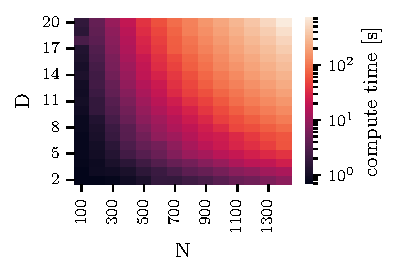
\includegraphics[width=0.47\textwidth]{fig/studies/wp_computational_cost/VWP}
  }
  \subcaptionbox{SVWP\label{fig:svwp-computational-complexity}}{
    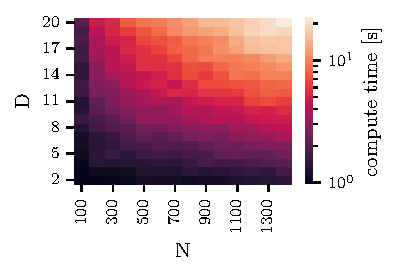
\includegraphics[width=0.47\textwidth]{fig/studies/wp_computational_cost/SVWP}
  }
  \caption{
    WP model training computational complexity as a function of number of time steps ($N$) and number of components ($D$).
    Shown is time required (in seconds) to complete~4 epochs.
    Run on a 3 GHz Intel Core i5 CPU.
  }\label{fig:wp-computational-cost}
\end{figure}


%%
\subsection{Implementation details}
%%

\info[inline]{Paragraph: Discuss implementational details.}
Throughout all benchmarks and experiments in this thesis, we use a (stationary, isotropic) Matérn 5/2 kernel, given by
\begin{equation}
  \label{eq:matern}
  k(\textbf{x}, \textbf{x}') = \sigma^2 (1 + \sqrt{5} r + \frac53 r^2) \exp(-\sqrt{5}r),
\end{equation}
with $r = \frac{||\textbf{x} - \textbf{x}'||}{l}$, and where $l$ and $\sigma$ are the kernel lengthscales and variance parameters, respectively, which are trained.
Their initial values are set to~0.3 and~1.0, respectively.
These parameters are part of the total set of model parameters~$\theta$.
This kernel is a twice differentiable covariance.
The popular radial basis function (RBF), also known as squared exponential or Gaussian, kernel is considered too smooth for our purposes (this kernel is infinitely differentiable), see \cref{fig:kernel-draws} as well.
We note that kernel choice imposes assumptions (i.e.~inductive bias) on the behavior of observed time series~\parencite[see also][chapter 2]{Duvenaud2014}.
For example, all Matérn kernels assume data stationarity.
Kernel functions can be considered as a specification of similarity between observations.
Our kernel considers further away observations less similar.
But a periodic kernel, for example, could consider a further away point \emph{more} similar if it is in phase with another point.
Or, as with the Gibbs kernel, kernel parameters could themselves be a function of input features $\mathbf{x}$ (e.g.~time).
In fact, this is one of the exciting aspects of the \gls{wp}.
We can characterize time series through these kernels.
The smoothness of correlation structures can be expressed by such kernel functions for example~\parencite{Fyshe2012, Fox2015, Foti2019}.
Kernels can be combined too; sums and products of kernels are also valid kernels.
As such more expressive kernels can be designed~\parencite{Gonen2011} and domain knowledge incorporated.
Kernel choice requires trial-and-error, although some efforts have been made to automate this process~\parencite[see e.g.][]{Steinruecken2019}.


\begin{figure}[t]
  \centering
  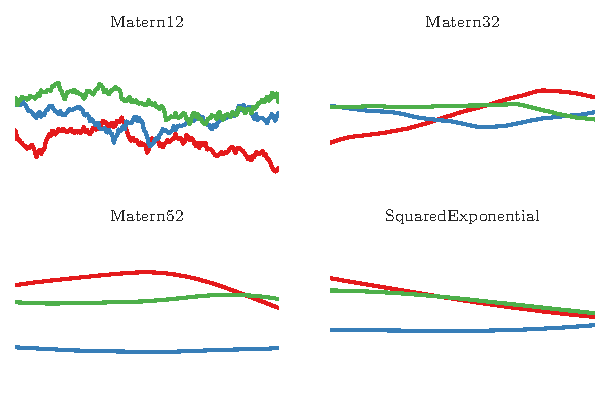
\includegraphics[width=\textwidth]{fig/studies/kernels}
  \caption{
    Draws from common Gaussian process kernels on interval $\left[ {0,1} \right]$.
  }\label{fig:kernel-draws}
\end{figure}


For all benchmarks and experiments we set $\nu = D$.
Larger values of $\nu$ have been tried empirically without improvement.
In general, it is best to keep $\nu$ small, as computational cost also scales with $\nu$.

We run both the \gls{vwp} and \gls{svwp} models in most experiments, although only the former for cases with $N \leq 200$ and only the latter for cases with $N \geq 400$.
The number of inducing points is set to $M = 200$, irrespective of time series lengths~$N$.

Standing on the shoulders of giants, the model is implemented using the open-source Python library \texttt{GPflow}~\parencite[][version 2.6.4]{Matthews2017, Wilk2020}.
This \gls{gp} toolbox in turn is built on top of Google's \texttt{Tensorflow}~\parencite[][version 2.11.0]{Tensorflow2015}.
These packages take care of all underlying automatic differentiation.
This means that the amount of code to write is minimal and consists mainly of implementing a (customized) likelihood function.
For these reasons, this black-box implementation~\parencite{Ranganath2014} is simple and fast compared to proposed inference routines based on \gls{mcmc}.
%
In fact, this is a crucial insight.
While we acknowledge the \gls{wp} as a complex model, and thus incur its accompanying cost, in return we get a favorable optimization routine that is robust and relatively straightforward.
Contrast this with the \gls{sw} approach, which is trivial in its description, but not straightforward in its implementation, with researchers facing many (arbitrary) implementational decisions to make.
Parameters are updated through gradient descent with Adam~\parencite{Kingma2015} with an initial learning rate of $\alpha = 0.001$.
All \gls{wp} \gls{tvfc} estimation figures in this thesis include the confidence interval of mean estimate plus/minus two standard deviations (i.e.~95\% of the mass of the \gls{wp}), based on 3,000 samples from the posterior.
